\chapter{Contexte et cadre du projet}

\section{Introduction}

Ce premier chapitre présente une vue d'ensemble du stage en exposant l'entreprise d'accueil et le contexte du projet COTS. Il établit le cadre contextuel nécessaire à la compréhension des enjeux multidimensionnels de cette mission de fin d'études, qui s'articule autour de :
\begin{itemize}
    \item La participation aux activités quotidiennes de développement
    \item L'implémentation spécialisée d'une plateforme d'automatisation des tests
\end{itemize}

Cette présentation contextuelle constitue le socle indispensable pour appréhender les dimensions technique, organisationnelle, sociétale et stratégique développées dans les chapitres suivants.

\section{Sopra Steria : Acteur majeur de la transformation numérique}

\subsection{Présentation générale et positionnement stratégique}

Sopra Steria s'impose comme un acteur européen majeur de la transformation numérique, fort de plus de 50 000 collaborateurs répartis dans 30 pays et s'appuyant sur plus de 50 ans d'expérience. L'entreprise se distingue par sa capacité à combiner une compréhension approfondie des enjeux métiers avec une expertise technologique de pointe.

En tant que leader du conseil, des services numériques et du développement logiciel, Sopra Steria accompagne les plus grandes organisations dans leurs projets de transformation à travers différents secteurs :
\begin{itemize}
    \item Transport et mobilité
    \item Finance et banque
    \item Secteur public et gouvernemental
    \item Industrie et énergie
\end{itemize}

\subsubsection{Indicateurs de performance}

Cette position de leadership se traduit par des indicateurs remarquables :

\begin{description}[leftmargin=3cm, labelwidth=2.5cm]
    \item[Chiffre d'affaires] Supérieur à 5 milliards d'euros, démontrant une performance financière solide et une croissance soutenue
    \item[Présence géographique] Dans 30 pays, soulignant sa portée internationale et sa capacité d'adaptation aux contextes locaux
    \item[Écosystème humain] Plus de 50 000 employés, reflétant des ressources substantielles et une diversité de compétences
    \item[Partenariats stratégiques] Avec les principaux fournisseurs technologiques et de solutions cloud du marché
    \item[Reconnaissance] Leader du conseil en transformation numérique par les grands analystes sectoriels
    \item[Portefeuille] Projets critiques réalisés avec succès pour les secteurs gouvernementaux et les grandes entreprises
\end{description}

\begin{figure}[H]
    \centering
    
\includegraphics[scale=0.8]{figures/sopra_presence_mondiale.png}
    \caption{Présence mondiale de Sopra Steria}
    \label{fig:sopra_presence}
\end{figure}

\subsubsection{Centre de Services de Nantes}

Le Centre de Services de Nantes représente un centre d'excellence spécialisé dans le domaine ferroviaire, caractérisé par :
\begin{itemize}
    \item Plus de 200 experts dédiés exclusivement aux projets SNCF
    \item Une concentration d'expertise permettant une collaboration étroite avec les équipes SNCF
    \item Un niveau de spécialisation technique et métier particulièrement élevé
    \item Une organisation en centres de compétences favorisant la mutualisation des connaissances
\end{itemize}

L'approche managériale se caractérise par un mélange de leadership collaboratif et d'excellence technique, favorisant un environnement où l'innovation est encouragée tout en maintenant des standards de qualité rigoureux.

\subsection{Mission, valeurs et approche différenciante}

\subsubsection{Mission stratégique}

La mission de Sopra Steria s'articule autour de l'accompagnement des organisations dans leur parcours de transformation numérique, selon trois axes fondamentaux :

\begin{description}
    \item[Excellence Numérique] Conception et déploiement de solutions numériques innovantes qui maximisent la valeur métier et l'efficacité opérationnelle des clients, adaptées aux spécificités sectorielles et organisationnelles
    \item[Leadership Technologique] Positionnement à la pointe de l'innovation technologique tout en garantissant des solutions pragmatiques, évolutives et alignées sur les besoins métiers réels
    \item[Partenariats Stratégiques] Construction de relations durables fondées sur la confiance, l'expertise conseil et la capacité de livraison fiable de projets complexes à forte criticité
\end{description}

\subsubsection{Système de valeurs}

L'approche différenciante repose sur un système de valeurs profondément ancré :

\begin{description}
    \item[Orientation Client] Compréhension approfondie des enjeux clients et adaptation des solutions aux défis spécifiques de chaque organisation, garantissant une réponse sur mesure aux problématiques métiers
    \item[Excellence Technique] Maintien de standards élevés en développement logiciel, architecture système et innovation technologique, assurant la qualité et la pérennité des solutions déployées
    \item[Collaboration Intégrée] Promotion du travail d'équipe et du partage de connaissances, tant en interne qu'avec les équipes clients, pour maximiser l'efficacité collective et la réussite des projets
    \item[Amélioration Continue] Encouragement du développement professionnel permanent et de la veille technologique pour rester en phase avec l'évolution rapide des technologies et des pratiques sectorielles
\end{description}

\subsection{Positionnement et intégration au sein du projet COTS}

Durant cette mission de stage, mon intégration s'est effectuée au sein de l'équipe projet COTS, selon l'organisation suivante :

\subsubsection{Encadrement}
\begin{itemize}
    \item \textbf{Pierre Mirat} - Chef de projet, supervision directe
    \item \textbf{Tom Richardson} - Tech Lead expérimenté du projet, collaboration technique étroite
\end{itemize}

\subsubsection{Équipe opérationnelle}
\begin{itemize}
    \item \textbf{Louis Legendre} et \textbf{Mélina Loyant} - Développeurs collaborateurs
    \item \textbf{Florian Carré} et \textbf{Marie-Émilie Deschez} - Analystes métier experts des processus SNCF
\end{itemize}

Cette organisation matricielle nécessite :
\begin{itemize}
    \item Des compétences organisationnelles développées
    \item Une capacité d'adaptation permanente
    \item Un équilibre efficace entre les contributions aux tâches de sprint récurrentes et l'avancement sur les objectifs spécialisés du projet d'automatisation
\end{itemize}

L'environnement collaboratif et la nature interdisciplinaire du projet COTS offrent une opportunité unique de travailler à l'intersection de :
\begin{itemize}
    \item L'ingénierie logicielle moderne
    \item L'expertise métier ferroviaire
    \item L'innovation en matière d'assurance qualité
\end{itemize}

\section{Le projet COTS : Modernisation du système d'information ferroviaire}

\subsection{Vision stratégique et architecture fonctionnelle}

Le projet COTS (Catalogue des Offres de Transport et de Services) constitue une initiative stratégique majeure de modernisation du système d'information de la SNCF. Cette plateforme unifiée vise à remplacer l'écosystème actuel composé de multiples systèmes patrimoniaux disparates par un référentiel centralisé et cohérent, capable de gérer l'intégralité des offres de transport et services associés.

\subsubsection{Principes de conception}

L'architecture du système COTS repose sur des principes modernes garantissant :

\begin{description}
    \item[Centralisation Intelligente] Consolidation des données d'offres de transport provenant de sources multiples en un référentiel unique faisant autorité, éliminant définitivement les silos informationnels et les incohérences de données
    \item[Évolutivité Architecturale] Conception modulaire permettant la gestion de volumes de données croissants et de charges utilisateur variables tout en maintenant des performances optimales et une fiabilité constante
    \item[Intégration Systémique] Interconnexion harmonieuse avec l'ensemble des systèmes SNCF existants et les plateformes partenaires externes via des APIs RESTful et des protocoles de messaging asynchrones robustes
    \item[Réactivité Temps Réel] Support natif des mises à jour de données temps réel et implémentation d'une architecture événementielle garantissant une réactivité immédiate aux changements opérationnels
    \item[Maintenabilité Avancée] Utilisation de patterns architecturaux éprouvés et de technologies modernes assurant la durabilité à long terme, la facilité de maintenance et l'évolutivité fonctionnelle
    \item[Conformité Réglementaire] Respect strict des standards de l'industrie ferroviaire et des exigences réglementaires nationales et européennes en matière de sécurité, fiabilité et protection des données
\end{description}

\subsubsection{Technologies clés}

L'architecture microservices actuelle s'appuie sur :
\begin{itemize}
    \item \textbf{Java Spring Boot} pour les services métiers
    \item \textbf{MongoDB} pour la persistance documentaire
    \item \textbf{Apache Kafka} pour le streaming de données
    \item \textbf{Architecture RESTful} pour les communications inter-services
\end{itemize}

\begin{figure}[H]
    \centering
    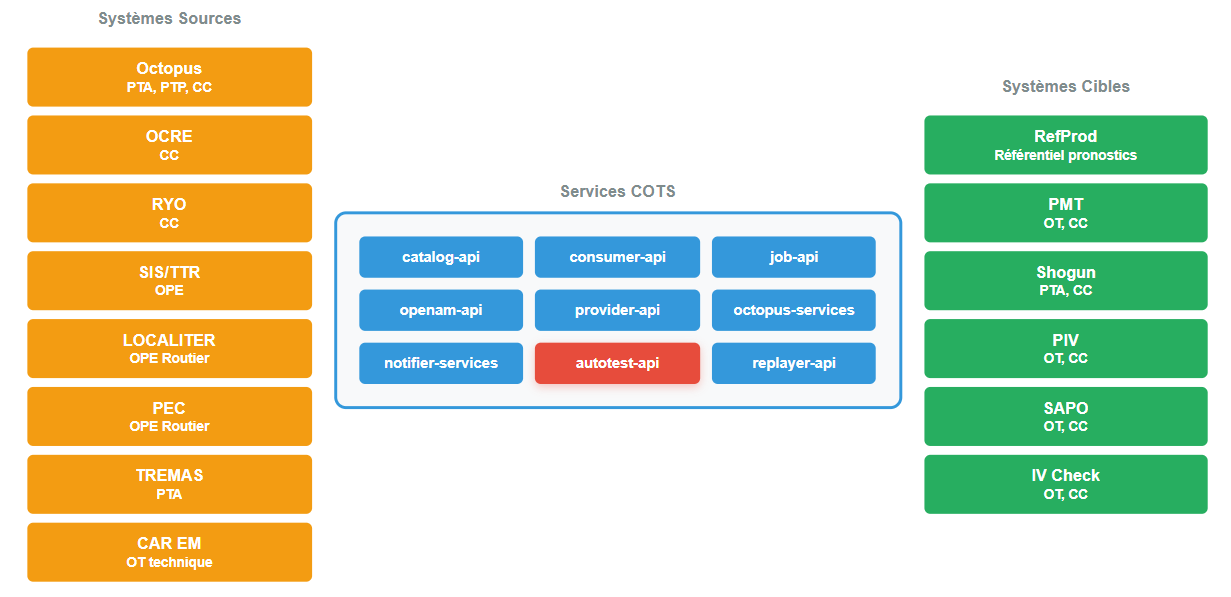
\includegraphics[scale=0.8]{figures/achitecture_cots.png}
    \caption{Architecture COTS - Microservices et Intégrations}
    \label{fig:architecture_cots}
\end{figure}

\subsection{Écosystème technique et services composants}

L'architecture microservices de COTS s'organise autour de neuf services critiques, chacun assumant des responsabilités spécifiques dans la chaîne de valeur du catalogue des offres :

\begin{description}
    \item[catalog-api] Service central de gestion des catalogues d'offres, responsable de la création, modification et orchestration du cycle de vie complet des offres de transport
    \item[consumer-api] Interface de consommation dédiée aux systèmes clients internes et externes, optimisant l'accès aux données du catalogue selon les profils utilisateurs
    \item[job-api] Orchestrateur de traitements batch et en temps réel, gérant l'exécution des processus métiers complexes et la synchronisation inter-systèmes
    \item[openam-api] Service d'authentification et d'autorisation sécurisée, intégrant les mécanismes de Single Sign-On et de gestion fine des droits d'accès
    \item[provider-api] Interface de fourniture de données vers les systèmes partenaires, assurant la diffusion contrôlée et sécurisée des informations catalogue
    \item[octopus-services] Ensemble de services métiers spécialisés, encapsulant la logique business complexe spécifique au domaine ferroviaire
    \item[notifier-services] Système de notification temps réel, gérant la diffusion d'événements et d'alertes vers les différents acteurs de l'écosystème
    \item[autotest-api] Service dédié à l'automatisation des tests, facilitant l'exécution de campagnes de validation et de non-régression
    \item[replayer-api] Système de rejeu de scénarios, permettant la reproduction et l'analyse de situations opérationnelles complexes
\end{description}

Cette architecture distribuée garantit :
\begin{itemize}
    \item Une séparation claire des responsabilités
    \item Une scalabilité horizontale optimale
    \item Une maintenabilité simplifiée
    \item La flexibilité nécessaire pour l'évolution future du système
\end{itemize}

\subsection{Domaines d'application et valeur métier}

La polyvalence fonctionnelle du système COTS lui permet de couvrir l'ensemble des processus métiers liés à la gestion des offres de transport SNCF, créant une valeur ajoutée significative dans plusieurs domaines critiques :

\subsubsection{Gestion des offres}
\begin{itemize}
    \item Centralisation de la création, modification et gestion du cycle de vie complet des offres de transport
    \item Couverture de l'ensemble des services SNCF (TGV, TER, Intercités)
    \item Processus harmonisés depuis la conception jusqu'au retrait des offres
\end{itemize}

\subsubsection{Optimisation économique}
\begin{itemize}
    \item Support des stratégies de tarification dynamique
    \item Optimisation des revenus grâce à une vision unifiée et temps réel
    \item Analyse de la demande client et ajustement des offres
\end{itemize}

\subsubsection{Excellence client}
\begin{itemize}
    \item Garantie d'une information d'offres cohérente, précise et actualisée
    \item Harmonisation à travers tous les points de contact client :
    \begin{itemize}
        \item Gares et bornes
        \item Plateformes web et mobile
        \item Centres d'appel
        \item Distributeurs partenaires
    \end{itemize}
\end{itemize}

\subsubsection{Écosystème partenarial}
\begin{itemize}
    \item Facilitation des échanges de données harmonieux avec les partenaires externes
    \item Intégration avec les agences de voyage
    \item Connexion aux plateformes de réservation tierces
    \item Support des systèmes de transport multimodaux
\end{itemize}

\subsection{Environnement concurrentiel et positionnement}

\subsubsection{Offre de services Sopra Steria}

Sopra Steria fournit des services complets pour répondre aux besoins clients dans le secteur transport :
\begin{itemize}
    \item Développement de solutions bout-en-bout
    \item Intégration système et services de maintenance continue
    \item Conseil technique et gestion de projet
    \item Formation et accompagnement à l'implémentation
\end{itemize}

\subsubsection{Différenciation concurrentielle}

Le projet COTS se distingue par :
\begin{itemize}
    \item Une approche sur mesure, spécifiquement adaptée aux exigences uniques de la SNCF
    \item La conformité aux contraintes réglementaires du secteur ferroviaire français
    \item Une personnalisation optimale pour le contexte ferroviaire français
    \item Une intégration harmonieuse avec l'infrastructure et les processus SNCF existants
\end{itemize}

\subsubsection{Perspectives d'évolution}

Les améliorations futures envisagées comprennent :
\begin{itemize}
    \item L'incorporation d'analytics avancés
    \item L'apprentissage automatique pour la prédiction de demande
    \item Des capacités de traitement temps réel améliorées
    \item L'extension des fonctionnalités de personnalisation client
\end{itemize}

\section{Enjeux et défis de la mission}

\subsection{Problématique de l'assurance qualité}

Les projets logiciels d'envergure comme COTS évoluent dans un contexte où l'assurance qualité constitue un défi majeur, particulièrement critique dans le domaine ferroviaire où la fiabilité et la sécurité sont impératives.

\subsubsection{Complexité des systèmes modernes}

La complexité croissante des systèmes distribués, couplée à l'accélération des cycles de développement agiles, exacerbe les difficultés traditionnelles :
\begin{itemize}
    \item Interdépendances complexes entre microservices
    \item Gestion de la cohérence des données distribuées
    \item Validation de bout en bout des parcours utilisateur
    \item Maintien de la performance sous charge variable
\end{itemize}

\subsubsection{Limitations de l'approche actuelle}

L'approche actuelle de tests de non-régression (TNR), réalisée manuellement via l'outil ALM (Application Lifecycle Management), révèle plusieurs limitations structurelles :

\begin{description}
    \item[Inefficience Temporelle] Exécution séquentielle et manuelle de chaque scénario de test, générant des cycles de validation particulièrement longs et incompatibles avec les contraintes de livraison continue
    \item[Vulnérabilité aux Erreurs] Manipulation manuelle des jeux de données et des paramètres de test, introduisant des risques d'erreur et d'incohérence dans les résultats de validation
    \item[Intensité Ressource] Mobilisation significative des équipes qualité sur des tâches répétitives, limitant leur disponibilité pour des activités à plus forte valeur ajoutée
    \item[Impact sur les Délais] Retards récurrents dans les cycles de déploiement dus aux contraintes temporelles des campagnes de test manuelles
    \item[Limitations de Traçabilité] Difficultés de suivi précis des résultats de test et de génération de rapports consolidés pour le pilotage qualité
\end{description}

\subsubsection{Défis spécifiques au projet COTS}

Le projet COTS fait spécifiquement face aux défis suivants :
\begin{itemize}
    \item Tests de régression suite aux mises à jour d'obsolescence
    \item Validation des efforts de modernisation système
    \item Maintien de la couverture de test complète avec l'augmentation de la complexité
    \item Assurance de la compatibilité inter-services lors des déploiements
\end{itemize}

\subsection{Objectifs de la mission et approche solution}

Cette mission de stage s'articule autour d'une double ambition : l'acquisition d'une expérience opérationnelle complète dans le développement logiciel d'entreprise et la contribution innovante à l'amélioration des processus d'assurance qualité du projet COTS.

\subsubsection{Objectifs spécifiques}

\begin{description}
    \item[Développement de Campagnes de Tests Automatisés] Conception et implémentation de scénarios de test complets utilisant le framework Cucumber pour le développement dirigé par le comportement (BDD), en collaboration étroite avec les analystes métier pour garantir la couverture exhaustive des exigences fonctionnelles
    \item[Intégration CI/CD Avancée] Configuration et déploiement de l'automatisation Jenkins pour l'exécution transparente des campagnes de test au sein du pipeline d'intégration continue, incluant la mise en place de seuils de qualité et de mécanismes de validation automatique
    \item[Optimisation du Pipeline de Déploiement] Intégration harmonieuse des tests automatisés dans les processus de déploiement pour assurer une validation systématique et fiable des nouvelles versions, réduisant significativement les risques de régression en production
\end{description}

\subsubsection{Bénéfices opérationnels attendus}

D'un point de vue opérationnel, cette mission vise à fournir :
\begin{itemize}
    \item Des capacités d'assurance qualité améliorées
    \item Une réduction de la charge de tests manuels
    \item Des cycles de feedback plus rapides
    \item Une confiance de release améliorée
    \item Un risque réduit de problèmes en production
    \item Une meilleure fiabilité système et satisfaction utilisateur
\end{itemize}

\subsection{Méthodologie et approche de mise en œuvre}

La réalisation de cette mission s'appuie sur une méthodologie agile adaptée, intégrant les principes Scrum avec les spécificités du développement de solutions de test automatisé.

\subsubsection{Structure méthodologique}

Cette approche se structure autour de six phases complémentaires et itératives :

\textbf{Phase 1 : Intégration et Analyse}
\begin{itemize}
    \item Immersion complète dans l'écosystème technique COTS (architecture, technologies, processus de développement)
    \item Analyse approfondie des pratiques de test existantes et identification des opportunités d'optimisation
    \item Maîtrise de la stack technologique (Java Spring Boot, MongoDB, Apache Kafka, Jenkins, outils de développement collaboratif)
\end{itemize}

\textbf{Phase 2 : Participation Opérationnelle}
\begin{itemize}
    \item Contribution active aux cérémonies agiles (daily standups, planification de sprint, rétrospectives d'amélioration continue)
    \item Participation aux développements fonctionnels, corrections d'anomalies et processus de revue de code collaborative
    \item Collaboration avec les analystes métier pour l'approfondissement de la compréhension des exigences fonctionnelles
\end{itemize}

\textbf{Phase 3 : Conception et Développement}
\begin{itemize}
    \item Architecture et implémentation du framework de tests automatisés basé sur Cucumber et les principes BDD
    \item Développement de l'infrastructure de test intégrée à l'application Spring Boot existante
    \item Création de bibliothèques de composants et d'utilitaires de test réutilisables pour maximiser l'efficacité et la maintenabilité
\end{itemize}

\textbf{Phase 4 : Intégration CI/CD}
\begin{itemize}
    \item Configuration avancée des jobs Jenkins pour l'orchestration automatisée des suites de tests
    \item Implémentation de quality gates intelligents et de procédures de gestion d'échec adaptatives
    \item Intégration transparente dans les workflows de déploiement existants
\end{itemize}

\textbf{Phase 5 : Validation et Optimisation}
\begin{itemize}
    \item Validation exhaustive de la plateforme avec des scénarios réels et des volumes de données représentatifs
    \item Optimisation des performances et de la fiabilité basée sur les résultats de test en conditions opérationnelles
    \item Vérification de l'alignement avec les objectifs initiaux et ajustements si nécessaire
\end{itemize}

\textbf{Phase 6 : Transfert et Pérennisation}
\begin{itemize}
    \item Création d'une documentation technique et fonctionnelle complète pour l'utilisation et la maintenance futures
    \item Formation approfondie des équipes et transfert de connaissances pour l'autonomie opérationnelle
    \item Capitalisation des enseignements et formulation de recommandations pour les évolutions futures
\end{itemize}

\subsubsection{Écosystème d'outils collaboratifs}

L'environnement de travail s'appuie sur :
\begin{itemize}
    \item \textbf{JIRA} pour la gestion agile et le suivi des issues
    \item \textbf{Confluence} pour la documentation et le partage de connaissances
    \item \textbf{Microsoft Teams} pour la communication quotidienne et les réunions virtuelles
    \item \textbf{Git} pour le contrôle de version et le développement collaboratif avec des processus de revue de code rigoureux
\end{itemize}

\section{Résumé}

Ce chapitre contextuel a établi les fondements nécessaires à la compréhension de la mission de stage dans toute sa complexité. Les éléments clés présentés incluent :

\begin{itemize}
    \item La présentation de Sopra Steria comme acteur majeur de la transformation numérique
    \item L'analyse détaillée du projet COTS et de ses enjeux stratégiques pour la SNCF
    \item La définition précise des objectifs et de la méthodologie de la mission
\end{itemize}

Ces éléments constituent le socle conceptuel indispensable pour appréhender les réalisations techniques et l'analyse multidimensionnelle développées dans les chapitres suivants. Cette approche contextuelle permet de saisir l'articulation entre :
\begin{itemize}
    \item Les contributions opérationnelles quotidiennes
    \item Le projet d'innovation spécialisé en automatisation de tests
\end{itemize}

Elle prépare ainsi l'analyse approfondie des dimensions technique, organisationnelle, environnementale et stratégique de cette expérience professionnelle enrichissante.